Durant le développement de nos différents clients, nous nous sommes rendus
compte que nous étions très limité par le temps de calcul. En effet,
la plupart de nos algorithmes n'étaient pas optimisés. Nous avons donc
eu recourt à du profilage

\subsection{Profilage et identification de zone critiques}
Après premier appel au profileur \textit{gprof} montré dans la Figure \ref{fig:gprof-find-neighbors}
, nous voyons déjà une première zone critique, \verb|find_neighbor_in_direction|.

\begin{figure}[H]
	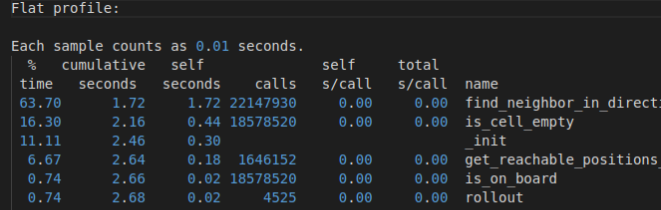
\includegraphics[width=\linewidth]{gprof_neighbors}
	\caption{Résultat du profileur \textit{gprof} après exécution d'une itération MCTS}
	\label{fig:gprof-find-neighbors}
\end{figure}

On remarque que la fonction \verb|find_neighbor_in_direction| nous mange
toute la puissance de calcul. Cette fonction est appelée plus de 22 millions de fois, elle 
occupe 63.70\% du temps CPU et la somme de la durée prise par tous ses appels est égale à 1.72 secondes, ce qui est gigantesque
pour une seule itération de MCTS. Au moment du profile, la fonction \verb|find_neighbor_in_direction| avait le fonctionnement défini
dans l'algorithme \ref{alg:find_neighbor_before}. Sa complexité était au moins de $O(nombre\_sommets)$ soit $O(n)$. Nous voudrions une complexité
$O(1)$ idéalement vu le nombre d'appels à cette fonction.

\begin{algorithm}
	\Entree{M: matrice d'adjacence, d: direction, i: $\mathbb{N} < nbre\_sommets$}
	\Deb{
		\PourTous{$0 \leq j < nbre\_sommets$}{
			\lSi{$M_{i,j} = dir$}{
				\Retour{j}
			}
		}
		\Retour{-1}\;
	}
	\caption{Algorithme peu efficace pour trouver le voisin dans une direction}
	\label{alg:find_neighbor_before}
\end{algorithm}

2 idées ont été implémentées pour améliorer cette méthode. Premièrement, on stocke le résultat
de l'algorithme dans un cache, donnant une complexité moyenne $O(1)$. Deuxièmement, la première approche
était très naïve, elle ne prenait pas en compte l'avantage du format CSR. En effet, avec le format CSR,
on peut tout simplement itérer sur les valeurs non zéros à la ligne $i$, ce qui équivaut à itérer sur tous
les voisins de $i$. Cette deuxième approche est de complexité $O(NUM\_DIRS)$, donc est aussi $O(1)$.
En fusionnant les deux approches, on peut obtenir l'algorithme \ref{alg:find_neighbor_opti} qui est très efficace
et prends avantage de nos structures de données.

\begin{algorithm}
	\Entree{M: matrice d'adjacence, d: direction, i: $\mathbb{N} < nbre\_sommets$}
	\Deb{
		\lSi{is\_neighbor\_cached(dir, i)}{
			\Retour{cached\_neighbor(dir, i)}
		}
		\PourCh{$j \in voisins(i)$}{
			\lSi{$M_{i,j} = dir$}{
				\Retour{j}
			}
		}
		\Retour{-1}\;
	}
	\caption{Algorithme peu efficace pour trouver le voisin dans une direction}
	\label{alg:find_neighbor_opti}
\end{algorithm}

Après application de ces résultats et un appel à \textit{gprof} affiché dans la Figure \ref{fig:gprof-empty-cell},
une nouvelle zone critique apparait: \emph{is\_cell\_empty}.
\begin{figure}[H]
	\centering
	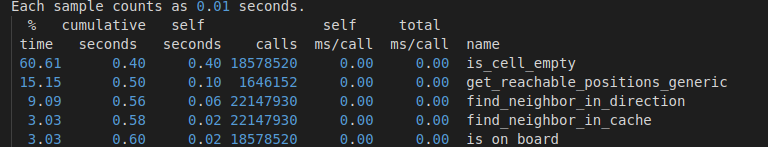
\includegraphics[width=\linewidth]{gprof_cell_empty}
	\captionsetup{justification=centering}
	\caption{Résultat du profileur \textit{gprof} après exécution d'une itération MCTS \\et optimisation \textit{find\_neighbor\_in\_direction}}
	\label{fig:gprof-empty-cell}
\end{figure}

Cette fois-ci, c'est \textit{is\_cell\_empty} qui occupe toutes les ressources CPU. La raison est simple,
nous stockons actuellement les positions des reines par joueur. Pour savoir si une case est vide,
il faut donc itérer sur toutes les reines de tous les joueurs pour savoir s'il y a une reine, et regarder s'il y a une flèche à cette position.
Là encore, nous avons un vilain $O(n)$ couplé à un nombre d'appels colossal. Cependant, la solution à ce problème
n'est pas si élégante que celle pour \textit{find\_neighbor\_in\_direction}. En effet,
nous devons dupliquer de l'information, car stocker les reines par joueur est intéressant pour d'autres algorithmes.
Nous avons donc décidé d'avoir une redondance de l'information, avec le champ \verb|queens| pour
avoir les positions des reines par joueur, et le champ \verb|queens_on_board| qui indique quelle reine est
à une position donnée en temps constant. Malheureusement, cela rajoute une complexité algorithmique aux fonctions \verb|apply_move| et \verb|cancel_move|
qui applique (resp. annule) un coup sur un plateau. Après optimisations et après changement de gprof à oprofile\footnote{gprof n'arrive pas à profile les librairies dynamiques, ce qui rendait le profiling pénible à effectuer. Nous avons donc opté pour oprofile qui permettait cela.},
nous obtenons la figure~\ref{fig:oprof-opti}, qui montre que nous avons encore quelques fonctions critiques, mais malheureusement nous
n'avons pas trouvé d'optimisations pertinentes à réaliser sur ces fonctions.

\begin{figure}[H]
	\centering
	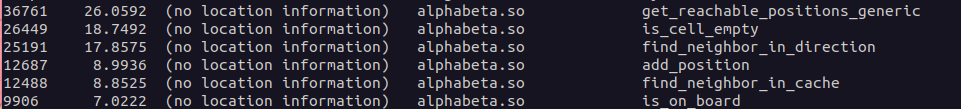
\includegraphics[width=\linewidth]{oprofile_opti}
	\captionsetup{justification=centering}
	\caption{Bilan oprofile d'une exécution d'une partie en utilisant la stratégie \emph{Function Deepening} de notre alphabeta}
\end{figure}